%!TEX root = ./main.tex

\section{Planning}
\addtocounter{minutes}{3}
\begin{frame}
	\frametitle{Planning}
    \includeSchedule
    
	% NOTE: Volgende sessie:  Dual boot $->$ USB stick en laptop

\end{frame}

\section{Blackboard}
\begin{frame}
    \frametitle{Blackboard}
    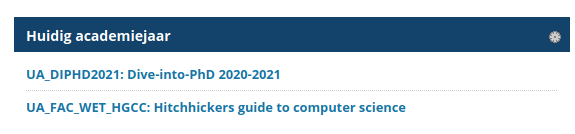
\includegraphics[scale=0.5]{res/bb.png}    

	
	Blackboard cursus Hitchhikers guide to computer science
	\vspace{1cm}

	Contacteer ons indien niet zichtbaar!\\
	\texttt{stijn.rosaer@student.uantwerpen.be}
\end{frame}

\section{Eerste sessie}
\begin{frame}
	\frametitle{Eerste sessie}
	\textbf{Donderdag 24 september}\\
	\vspace{1cm}
	
	\begin{center}
	\begin{tabular}{c|c|c}
    Groep A & G.004 & 9:30\\
    Groep B & G.005 & 9:30\\ \hline
    Groep C & G.004 & 16:00\\
    Groep D & G.005 & 16:00
    \end{tabular}
	\end{center}
    
\end{frame}







